\subsection{Métricas}

Para observar el comportamiento de los algoritmos de $scheduling$ no basta con hacer un gráfico, también hay que poder extraer información de él y así realizar un análisis del rendimiento de algoritmo. Esa informaci\'on tiene que poder ser cuatificable, ya que si lo fuese podr\'iamos utilizar esta informaci\'on para comparar varios algoritmos y decidir cu\'al es el m\'as conveniente seg\'un un conjunto determinado de procesos. Por ello recurrimos al uso de m\'etricas, para poder obtener n\'umeros a partir de una corrida determinada de un algoritmo de $scheduling$. Las m\'etricas nos permitir\'an decidir si el algoritmo est\'a aportando a cumplir algunos de los objetivos indicados anteriormente en la introducci\'on. Tanembaum\cite{Tanen} propone una divisi\'on entre el tipo de tareas posibles, en base a sus caracter\'isticas, a saber:

Tipos de tareas:
\begin{itemize}
	\item $Batch$ o de lotes, que se caracterizan por utilizar mucho el CPU, de manera continua y con pocos accesos a dispositivos de entrada y salida.
	\item $Interactive$ o interactivos, que particularmente usan mucho los dispositivos de entrada y salida.  
\end{itemize}

Los conjuntos de tareas que utilizamos para probar los algoritmos de $scheduling$ en el simulador generalmente poseen ambos tipos de tareas, as\'i que haremos un an\'alisis bastante general cu\'ales m\'etricas aplicar.

Nos parece de principal inter\'es analizar las siguientes m\'etricas.

\subsubsection{Turn-around time}

$Turn-around$ $time$($TAT$) se define como el tiempo que tarda un proceso en terminar desde que est\'a listo para ejecutarse. Si un proceso se ejecuta desde el principio, entonces el n\'umero coinicide con tiempo total que tard\'o en terminar. Notemos que este tiempo no puede ser menor al tiempo total de ejecuci\'on; no tiene sentido que una tarea termine antes de ejecutar todo lo que deb\'ia ejecutar. Podemos medir entonces el $turn-around$ $time$  %%%%%%       Analicemos el $turn-around$ $time$ para los distintos algoritmos de $scheduling$ vistos:

\paragraph{FCFS}

En este algoritmo, nuestra intuici\'on nos dice que el $turn-around time$ de las tareas resultar\'a ser malo, ya que su ejecuci\'on depende de que otros procesos terminen el suyo ya que no hay posibilidad de ejecuci\'on de procesos en paralelo, al menos con un sólo núcleo.

\begin{figure}
	
\end{figure}



Se puede probar que, dado un conjunto $\{P_{i}\}_{0 < n}$ tareas, cada una con un tiempo de procesamiento $t_{i}$ con $i$ $\in$ [$0$,$n-1$] y un tiempo de llegada $s_{i}$ con $i$ $\in$ [$0$, $n-1$]. Suponiendo que $s_{i}$ $\leq$ $s_{j}$ para $i$ < $j$ (los tiempos de llegada están ordenados de mayor a menor) entonces vale que el $TAT$ de la $i$-ésima tarea resultará:

\begin{align*}
TAT(P_{i}) = max\left(\sum_{p=0}^{i-1}t_{p} - s_{i}, 0\right) + t_{i}
\end{align*}

Viendo esta ecuación vemos que el $TAT$ depende de el tiempo de procesamiento de las tareas anteriores. Por lo tanto, minimizando ese valor obtendríamos un $TAT$ mínimo. Este mínimo es alcanzado cuando el orden de llegada de las tareas es en base al tiempo de procesamiento en orden ascendente. Pero en la práctica esto no sucede
  
\begin{figure}
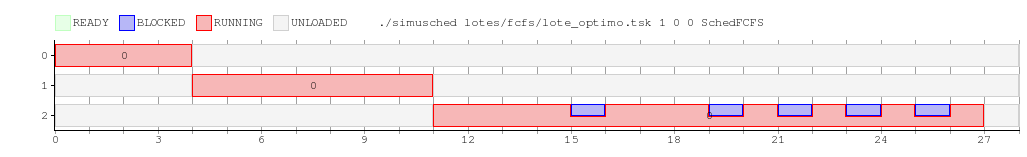
\includegraphics[scale=0.4]{FCFS/optimo2.png}
\caption{Ejemplo donde $FCFS$ es óptimo y el $TAT$ coincide con el tiempo de procesamiento}
\end{figure}


\subsubsection{Response time}
